%%%%%%%%%%%%%%%%%%%%%%%%%%%%%%%%%%%%%%%%%
% Masters/Doctoral Thesis 
% LaTeX Template
%
% This template was downloaded from:
% http://www.LaTeXTemplates.com
%
% Version 2.x major modifications by:
% Vel (vel@latextemplates.com)
%
% Original Authors:
% Vel (vel@latextemplates.com)
% Johannes Böttcher
% Steve Gunn (http://users.ecs.soton.ac.uk/srg/softwaretools/document/templates/)
% Sunil Patel (http://www.sunilpatel.co.uk/thesis-template/)
%
% This template was modified by Muneendra Ojha to suit the needs of 
% IIIT Allahabad Students. This is a basic template consisting of all 
% requirements as approved by the institute. Please feel free to contact
% if any errors are found or updates needed.
% 
% Do not remove this preamble. Always remember to give credits where it is due.
% 
% Template license:
% CC BY-NC-SA 3.0 (http://creativecommons.org/licenses/by-nc-sa/3.0/)
%
%%%%%%%%%%%%%%%%%%%%%%%%%%%%%%%%%%%%%%%%%

%----------------------------------------------------------------------------------------
%	PACKAGES AND OTHER DOCUMENT CONFIGURATIONS
%----------------------------------------------------------------------------------------

\documentclass[
12pt, % The default document font size, options: 10pt, 11pt, 12pt
oneside, % Two side (alternating margins) for binding by default, uncomment to switch to one side
english, % ngerman for German
singlespacing, % options: singlespacing, onehalfspacing or doublespacing
%draft, % Uncomment to enable draft mode (no pictures, no links, overfull hboxes indicated)
% nolistspacing, % If the document is onehalfspacing or doublespacing, uncomment this to set spacing in lists to single
liststotoc, % Uncomment to add the list of figures/tables/etc to the table of contents
% toctotoc, % Uncomment to add the main table of contents to the table of contents
parskip, % Uncomment to add space between paragraphs
%nohyperref, % Uncomment to not load the hyperref package
headsepline, % Uncomment to get a line under the header
% chapterinoneline, % Uncomment to place the chapter title next to the number on one line
% consistentlayout, % Uncomment to change the layout of the declaration, abstract and acknowledgements pages to match the default layout
]{Thesis} % The class file specifying the document structure



\usepackage[utf8]{inputenc} % Required for inputting international characters
\usepackage[T1]{fontenc} % Output font encoding for international characters
\usepackage{mathpazo} % Use the Palatino font by default
\usepackage[backend=biber,
style=numeric,
bibencoding=utf8,
% style=authoryear, % if using style as authoryear, then cite the reference using \parencite{}
% style=reading
]{biblatex}
\addbibresource{example.bib} % The filename of the bibliography
\usepackage[autostyle=true]{csquotes} % Required to generate language-dependent quotes in the bibliography
\usepackage{array}% http://ctan.org/pkg/array
\usepackage{lipsum}



%----------------------------------------------------------------------------------------
%	MARGIN SETTINGS
%----------------------------------------------------------------------------------------

\geometry{
	paper=a4paper, % Change to letterpaper for US letter
	inner=20mm, % Inner margin
	outer=20mm, % Outer margin
	bindingoffset=5mm, % Binding offset
	top=25mm, % Top margin
	bottom=20mm, % Bottom margin
	%showframe, % Uncomment to show how the type block is set on the page
}


%----------------------------------------------------------------------------------------
%	★★★ FILL IN YOUR INFORMATION HERE ★★★
%   THIS IS THE ONLY SECTION YOU NEED TO EDIT!
%----------------------------------------------------------------------------------------

% ============================================================
% THESIS DETAILS
% ============================================================
\thesistitle{Title of the thesis being submitted}
\degree{Bachelor of Technology}  % Options: Bachelor of Technology, Master of Technology, Doctor of Philosophy

% ============================================================
% SUPERVISOR DETAILS
% ============================================================
\supervisor{Dr. Supervisor Name}

% ============================================================
% STUDENT 1 DETAILS (Required - at least one student)
% ============================================================
\newcommand{\studentonename}{Student - 1}
\newcommand{\studentoneroll}{IIT2021001}

% ============================================================
% STUDENT 2 DETAILS (Optional - comment out if only 1 student)
% ============================================================
\newcommand{\studenttwoname}{Student - 2}
\newcommand{\studenttworoll}{IIT2021002}

% ============================================================
% STUDENT 3 DETAILS (Optional - comment out if only 2 students)
% ============================================================
\newcommand{\studentthreename}{Student - 3}
\newcommand{\studentthreeroll}{IIT2021003}

% ============================================================
% DEPARTMENT & UNIVERSITY (Usually don't need to change)
% ============================================================
\department{Department of Information Technology}
\university{Indian Institute of Information Technology, Allahabad}
\subject{Information Technology}

% ============================================================
% HELPER COMMANDS - DO NOT EDIT BELOW THIS LINE
% These automatically format the student information
% ============================================================

% Format for title page (with line breaks)
\newcommand{\studentnamesformatted}{%
\studentonename%
\ifdefined\studenttwoname%
\\\studenttwoname%
\fi%
\ifdefined\studentthreename%
\\\studentthreename%
\fi%
}

\newcommand{\rollnumbersformatted}{%
\studentoneroll%
\ifdefined\studenttworoll%
\\\studenttworoll%
\fi%
\ifdefined\studentthreeroll%
\\\studentthreeroll%
\fi%
}

% Format for certificate (comma separated)
\newcommand{\studentnamescomma}{%
\studentonename%
\ifdefined\studenttwoname%
, \studenttwoname%
\fi%
\ifdefined\studentthreename%
, \studentthreename%
\fi%
}

% Format for declaration (with roll numbers)
\newcommand{\studentnamesdeclaration}{%
\studentonename{} (\studentoneroll)%
\ifdefined\studenttwoname%
, \studenttwoname{} (\studenttworoll)%
\fi%
\ifdefined\studentthreename%
, and \studentthreename{} (\studentthreeroll)%
\fi%
}

% Format for signatures
\newcommand{\studentsignatures}{%
\studentonename{} (\studentoneroll)%
\ifdefined\studenttwoname%
\\\studenttwoname{} (\studenttworoll)%
\fi%
\ifdefined\studentthreename%
\\\studentthreename{} (\studentthreeroll)%
\fi%
}

% Pronoun selection (I/We)
\newcommand{\pronounwe}{%
\ifdefined\studenttwoname%
We%
\else%
I%
\fi%
}

\newcommand{\pronounus}{%
\ifdefined\studenttwoname%
us%
\else%
me%
\fi%
}

% Legacy compatibility
\firstauthor{\studentnamesformatted}
\enrollmentnumber{\rollnumbersformatted}

% ============================================================
% END OF USER CONFIGURATION
% ============================================================

\examiner{} 
\addresses{} 
\keywords{} 
\faculty{Faculty Name}



\AtBeginDocument{
\hypersetup{pdftitle=\ttitle} % Set the PDF's title to your title
% \hypersetup{pdfauthor=\authorname} % Set the PDF's author to your name
\hypersetup{pdfkeywords=\keywordnames} % Set the PDF's keywords to your keywords
}


\begin{document}
\begin{sloppypar}

%----------------------------------------------------------------------------------------
%	FRONT CONTENT
%----------------------------------------------------------------------------------------

\frontmatter% Use roman page numbering style (i, ii, iii, iv...) for the pre-content pages

\pagestyle{plain} % Default to the plain heading style until the thesis style is called for the body content
%----------------------------------------------------------------------------------------
%	TITLE PAGE
%----------------------------------------------------------------------------------------

\begin{titlepage}
\begin{center}
\begin{spacing}{1.2}

{\huge \bfseries \ttitle\par}  % ← Uses thesis title from main.tex

\vspace {5mm}
\textit{A thesis submitted in partial fulfillment of the requirements\\for the award of the degree of} 

\vspace{7mm}
\textsc{\huge \MakeUppercase{\degreename}}  % ← Uses degree from main.tex

\vspace {3mm}
% Logo display - no figure environment needed on title page

\includegraphics[width=5cm]{Figures/IIITA_Logo.png}
\vspace{5mm}

% ************************************
\begin{minipage}[t]{0.5\textwidth}
    \begin{flushleft} \large
        \textit{By:-} \\%[2mm]
            \textsc{\studentnamesformatted} % ← Uses student names from main.tex
    \end{flushleft}
\end{minipage}
\begin{minipage}[t]{0.45\textwidth}
    \begin{flushright} \large
        \textit{Enrollment No.} \\
            \textsc{\rollnumbersformatted} % ← Uses roll numbers from main.tex
    \end{flushright}
\end{minipage}\\[1cm]
% *************************************

\textit{Under the Supervision of}\\[2mm]
\textsc{\Large \supname}\\% ← Uses supervisor name from main.tex
\vspace{7mm}
\textit{Submitted to the}\\[2mm]
\textsc{\Large \deptname}\\ % ← Uses department from main.tex

\vspace{15mm}
\begin{hindi}
    {\Large\textsc{
        भारतीय सूचना प्रौद्योगिकी संस्थान, इलाहाबाद
    }}
\end{hindi} \\[3mm]
\textsc{\Large \univname} % ← Uses university from main.tex

\vspace{5mm}
\monthyear


\end{spacing}
\end{center}
\end{titlepage}


%----------------------------------------------------------------------------------------
%	CERTIFICATE
%----------------------------------------------------------------------------------------
\checktoopen
\begin{figure}[htp]
    % \centering
    
\includegraphics[height=3cm,keepaspectratio]{Figures/IIITA_Header.png}
\end{figure}
\thispagestyle{empty}
% \vspace*{.06\textheight}

\begin{spacing}{1.5}
\begin{center}
    {\centering\large\bfseries CERTIFICATE \par\vspace{10pt}}
\end{center}

\noindent It is certified that the work contained in the thesis titled \enquote{\ttitle} by {\studentnamescomma} has been carried out under my supervision and that this work has not been submitted elsewhere for a degree.
% ↑ Uses title and student names from main.tex

\vspace{3.5cm}
\hfill\begin{minipage}{7.5cm}   %{0.52\linewidth}
    \begin{spacing}{1.2}
        \par
        \rule{\textwidth}{0.2pt}\\
        {\supname} \par  % ← Uses supervisor name from main.tex
        {\deptname}  \par  % ← Uses department from main.tex
        IIIT Allahabad \par
    \end{spacing}
\end{minipage}

\end{spacing}
% \end{certificate}
\cleardoublepage

%----------------------------------------------------------------------------------------
%	DECLARATION
%----------------------------------------------------------------------------------------
\checktoopen
\begin{figure}[htp]
    % \centering
    
\includegraphics[height=3cm,keepaspectratio]{Figures/IIITA_Header.png}
\end{figure}
% \string\setblankpagestyle \space
\thispagestyle{empty}
\vspace{1mm}

\begin{center}
    {\large\bfseries CANDIDATE DECLARATION}
\end{center}

\begin{spacing}{1.2}

\noindent \pronounwe, \studentnamesdeclaration, hereby certify that the thesis titled \enquote{\ttitle} has been submitted by \pronounus{} in partial fulfillment of the requirements for the Degree of \degreename{} in the \deptname{} at the \univname.
% ↑ Uses pronouns and names from main.tex - automatically adjusts for single/multiple students

\par
\noindent We acknowledge that plagiarism includes: 
\begin{enumerate} 
    \item Reproducing another person's work (fully or partially) or ideas and presenting them as our own.
    \item Copying or paraphrasing another person's work without appropriate attribution.
    \item Engaging in literary theft by reproducing a unique literary construct without crediting its source.
\end{enumerate}
\par
We affirm that due credit has been given to all original authors and sources through proper citations for words, ideas, diagrams, graphics, computer programs, experiments, results, and websites that are not our own contributions. Direct quotations have been appropriately marked, and sources have been properly referenced. Furthermore, we declare that no portion of our work is plagiarized. In the event of a plagiarism claim, we accept full responsibility for the contents of this thesis. We acknowledge that our supervisor may not be able to verify the originality of every aspect of our work.
\end{spacing}

\begin{spacing}{2.0}
% \vspace{1cm}
\noindent
\begin{minipage}[t]{0.4\textwidth}  
    \begin{flushleft} 
        Place: \rule{40mm}{0.1pt}\\
    \end{flushleft}
\end{minipage}
\hfill
\begin{minipage}[t]{0.4\textwidth}
    \begin{flushright}         
        Date: \rule{40mm}{0.1pt}\\       
    \end{flushright}
\end{minipage}
% \rule{\textwidth}{0.1pt}\\
\par
{\studentsignatures} % ← Uses student names and rolls from main.tex
\end{spacing}


        
\cleardoublepage



%----------------------------------------------------------------------------------------
%	QUOTATION PAGE
%----------------------------------------------------------------------------------------

% \vspace*{0.2\textheight}
% \begin{spacing}{1.5}
% \noindent\enquote{\itshape Thanks to my solid academic training, today I can write hundreds of words on virtually any topic without possessing a shred of information, which is how I also got a good job in industry.}\bigbreak

% \hfill {\firstauthorname}
% \end{spacing}
% \cleardoublepage


%----------------------------------------------------------------------------------------
%	ABSTRACT PAGE
%----------------------------------------------------------------------------------------

\begin{abstract}
\begin{spacing}{2}

\addchaptertocentry{\abstractname} % Add the abstract to the table of contents
A B.Tech thesis should contain an abstract not exceeding 300 words (about one page), and a Ph.D thesis should contain an abstract synopsis not exceeding 1000 words (about four pages) in double spacing. Some random text is written as a sample.

\lipsum[1]


\end{spacing}
\end{abstract}

%----------------------------------------------------------------------------------------
%	ACKNOWLEDGEMENTS
%----------------------------------------------------------------------------------------

\begin{acknowledgements}
\begin{spacing}{1.5}
\addchaptertocentry{\acknowledgementname} % Add the acknowledgements to the table of contents

The acknowledgments and the people to thank go here, don't forget to include your project advisor\ldots

\lipsum[1]
\end{spacing}
\end{acknowledgements}

%----------------------------------------------------------------------------------------
%	LIST OF CONTENTS/FIGURES/TABLES PAGES
%----------------------------------------------------------------------------------------

\tableofcontents % Prints the main table of contents

\listoffigures % Prints the list of figures


\listoftables % Prints the list of tables


%----------------------------------------------------------------------------------------
%	ABBREVIATIONS
%----------------------------------------------------------------------------------------

\begin{abbreviations}{ll} % Include a list of abbreviations (a table of two columns)

\textbf{LAH} & \textbf{L}ist \textbf{A}bbreviations \textbf{H}ere\\
\textbf{WSF} & \textbf{W}hat (it) \textbf{S}tands \textbf{F}or\\

\end{abbreviations}

%----------------------------------------------------------------------------------------
%	PHYSICAL CONSTANTS/OTHER DEFINITIONS
%----------------------------------------------------------------------------------------

\begin{constants}{lr@{${}={}$}l} % The list of physical constants is a three column table

% The \SI{}{} command is provided by the siunitx package, see its documentation for instructions on how to use it

Speed of Light & $c_{0}$ & \SI{2.99792458e8}{\meter\per\second} (exact)\\
Constant Name & $Symbol$ & $Constant Value$ with units\\

\end{constants}

%----------------------------------------------------------------------------------------
%	SYMBOLS
%----------------------------------------------------------------------------------------

\begin{symbols}{lll} % Include a list of Symbols (a three column table)

$a$ & distance & \si{\meter} \\
$P$ & power & \si{\watt} (\si{\joule\per\second}) \\
%Symbol & Name & Unit \\

\addlinespace % Gap to separate the Roman symbols from the Greek

$\omega$ & angular frequency & \si{\radian} \\

\end{symbols}

%----------------------------------------------------------------------------------------
%	DEDICATION
%----------------------------------------------------------------------------------------

\dedicatory{For/Dedicated to/To my\ldots} 


%----------------------------------------------------------------------------------------
%	THESIS CONTENT - CHAPTERS
%----------------------------------------------------------------------------------------

\mainmatter % Begin numeric (1,2,3...) page numbering

\pagestyle{thesis} % Return the page headers back to the "thesis" style
\begin{spacing}{2}
    

% Include the chapters of the thesis as separate files from the Chapters folder
% Uncomment the lines as you write the chapters

% Chapter 1

\chapter{Introduction} % Main chapter title

\label{Chapter1} % For referencing the chapter elsewhere, use \ref{Chapter1} 

%----------------------------------------------------------------------------------------

% Define some commands to keep the formatting separated from the content 
\newcommand{\keyword}[1]{\textbf{#1}}
\newcommand{\tabhead}[1]{\textbf{#1}}
\newcommand{\code}[1]{\texttt{#1}}
\newcommand{\file}[1]{\texttt{\bfseries#1}}
\newcommand{\option}[1]{\texttt{\itshape#1}}

%----------------------------------------------------------------------------------------
% \addchaptertocentry{ABSTRACT}
% \begin{center}
%     {\centering\large\bfseries ABSTRACT}
% \end{center}
Provide a short one paragraph introduction about the chapter in 100 to 150  words. This chapter provides the overall introduction to the work presented in this thesis. Explain something about what is written in each section and what is the overall layout of this chapter. If you are writing a thesis (or will be in the future) and its subject is technical or mathematical (though it doesn't have to be), then creating it in \LaTeX{} is highly recommended as a way to make sure you can just get down to the essential writing without having to worry over formatting.

% \newpage

%----------------------------------------------------------------------------------------

%----------------------------------------------------------------------------------------

\section{Welcome and Thank You}
Welcome to this \LaTeX{} Thesis Template, a beautiful and easy to use template for writing a thesis using the \LaTeX{} typesetting system.

If you are writing a thesis (or will be in the future) and its subject is technical or mathematical (though it doesn't have to be), then creating it in \LaTeX{} is highly recommended as a way to make sure you can just get down to the essential writing without having to worry over formatting or wasting time arguing with your word processor.

\LaTeX{} is easily able to professionally typeset documents that run to hundreds or thousands of pages long. With simple mark-up commands, it automatically sets out the table of contents, margins, page headers and footers and keeps the formatting consistent and beautiful. One of its main strengths is the way it can easily typeset mathematics, even \emph{heavy} mathematics. Even if those equations are the most horribly twisted and most difficult mathematical problems that can only be solved on a super-computer, you can at least count on \LaTeX{} to make them look stunning.

%----------------------------------------------------------------------------------------

\section{Learning \LaTeX{}}

\LaTeX{} is not a \textsc{wysiwyg} (What You See is What You Get) program, unlike word processors such as Microsoft Word or Apple's Pages. Instead, a document written for \LaTeX{} is actually a simple, plain text file that contains \emph{no formatting}. You tell \LaTeX{} how you want the formatting in the finished document by writing in simple commands amongst the text, for example, if I want to use \emph{italic text for emphasis}, I write the \verb|\emph{text}| command and put the text I want in italics in between the curly braces. This means that \LaTeX{} is a \enquote{mark-up} language, very much like HTML.

\subsection{A (not so short) Introduction to \LaTeX{}}

If you are new to \LaTeX{}, there is a very good eBook -- freely available online as a PDF file -- called, \enquote{The Not So Short Introduction to \LaTeX{}}. The book's title is typically shortened to just \emph{lshort}. You can download the latest version (as it is occasionally updated) from here:
\url{http://www.ctan.org/tex-archive/info/lshort/english/lshort.pdf}

It is also available in several other languages. Find yours from the list on this page: \url{http://www.ctan.org/tex-archive/info/lshort/}

It is recommended to take a little time out to learn how to use \LaTeX{} by creating several, small `test' documents, or having a close look at several templates on:\\ 
\url{http://www.LaTeXTemplates.com}\\ 
Making the effort now means you're not stuck learning the system when what you \emph{really} need to be doing is writing your thesis.

\subsection{A Short Math Guide for \LaTeX{}}

If you are writing a technical or mathematical thesis, then you may want to read the document by the AMS (American Mathematical Society) called, \enquote{A Short Math Guide for \LaTeX{}}. It can be found online here:
\url{http://www.ams.org/tex/amslatex.html}
under the \enquote{Additional Documentation} section towards the bottom of the page.

\subsection{Common \LaTeX{} Math Symbols}
There are a multitude of mathematical symbols available for \LaTeX{} and it would take a great effort to learn the commands for them all. The most common ones you are likely to use are shown on this page:
\url{http://www.sunilpatel.co.uk/latex-type/latex-math-symbols/}

You can use this page as a reference or crib sheet, the symbols are rendered as large, high quality images so you can quickly find the \LaTeX{} command for the symbol you need.

\subsection{\LaTeX{} on a Mac}
 
The \LaTeX{} distribution is available for many systems including Windows, Linux and Mac OS X. The package for OS X is called MacTeX and it contains all the applications you need -- bundled together and pre-customized -- for a fully working \LaTeX{} environment and work flow.
 
MacTeX includes a custom dedicated \LaTeX{} editor called TeXShop for writing your `\file{.tex}' files and BibDesk: a program to manage your references and create your bibliography section just as easily as managing songs and creating playlists in iTunes.

%----------------------------------------------------------------------------------------

\section{Getting Started with this Template}

If you are familiar with \LaTeX{}, then you should explore the directory structure of the template and then proceed to place your own information into the \emph{THESIS INFORMATION} block of the \file{main.tex} file. You can then modify the rest of this file to your unique specifications based on your degree/university. Section \ref{FillingFile} on page \pageref{FillingFile} will help you do this. Make sure you also read section \ref{ThesisConventions} about thesis conventions to get the most out of this template.

If you are new to \LaTeX{} it is recommended that you carry on reading through the rest of the information in this document.

Before you begin using this template you should ensure that its style complies with the thesis style guidelines imposed by your institution. In most cases this template style and layout will be suitable. If it is not, it may only require a small change to bring the template in line with your institution's recommendations. These modifications will need to be done on the \file{Thesis.cls} file.

\subsection{About this Template}

This \LaTeX{} Thesis Template is originally based and created around a \LaTeX{} style file created by Steve R.\ Gunn from the University of Southampton (UK), Department of Electronics and Computer Science. You can find his original thesis style file at his site, here:
\url{http://www.ecs.soton.ac.uk/~srg/softwaretools/document/templates/}

Steve's \file{ecsthesis.cls} was then taken by Sunil Patel who modified it by creating a skeleton framework and folder structure to place the thesis files in. The resulting template can be found on Sunil's site here:
\url{http://www.sunilpatel.co.uk/thesis-template}

Sunil's template was made available through \url{http://www.LaTeXTemplates.com} where it was modified many times based on user requests and questions. Version 2.0 and onwards of this template represents a major modification to Sunil's template and is, in fact, hardly recognisable. The work to make version 2.0 possible was carried out by \href{mailto:vel@latextemplates.com}{Vel} and Johannes Böttcher.

%----------------------------------------------------------------------------------------

\section{What this Template Includes}

\subsection{Folders}

This template comes as a single zip file that expands out to several files and folders. The folder names are mostly self-explanatory:

\keyword{Appendices} -- this is the folder where you put the appendices. Each appendix should go into its own separate \file{.tex} file. An example and template are included in the directory.

\keyword{Chapters} -- this is the folder where you put the thesis chapters. A thesis usually has about six chapters, though there is no hard rule on this. Each chapter should go in its own separate \file{.tex} file and they can be split as:
\begin{itemize}
\item Chapter 1: Introduction to the thesis topic
\item Chapter 2: Background information and theory
\item Chapter 3: (Laboratory) experimental setup
\item Chapter 4: Details of experiment 1
\item Chapter 5: Details of experiment 2
\item Chapter 6: Discussion of the experimental results
\item Chapter 7: Conclusion and future directions
\end{itemize}
This chapter layout is specialised for the experimental sciences, your discipline may be different.

\keyword{Figures} -- this folder contains all figures for the thesis. These are the final images that will go into the thesis document.

\subsection{Files}

Included are also several files, most of them are plain text and you can see their contents in a text editor. After initial compilation, you will see that more auxiliary files are created by \LaTeX{} or BibTeX and which you don't need to delete or worry about:

\keyword{example.bib} -- this is an important file that contains all the bibliographic information and references that you will be citing in the thesis for use with BibTeX. You can write it manually, but there are reference manager programs available that will create and manage it for you. Bibliographies in \LaTeX{} are a large subject and you may need to read about BibTeX before starting with this. Many modern reference managers will allow you to export your references in BibTeX format which greatly eases the amount of work you have to do.

\keyword{Thesis.cls} -- this is an important file. It is the class file that tells \LaTeX{} how to format the thesis. 

\keyword{main.pdf} -- this is your beautifully typeset thesis (in the PDF file format) created by \LaTeX{}. It is supplied in the PDF with the template and after you compile the template you should get an identical version.

\keyword{main.tex} -- this is an important file. This is the file that you tell \LaTeX{} to compile to produce your thesis as a PDF file. It contains the framework and constructs that tell \LaTeX{} how to layout the thesis. It is heavily commented so you can read exactly what each line of code does and why it is there. After you put your own information into the \emph{THESIS INFORMATION} block -- you have now started your thesis!

Files that are \emph{not} included, but are created by \LaTeX{} as auxiliary files include:

\keyword{main.aux} -- this is an auxiliary file generated by \LaTeX{}, if it is deleted \LaTeX{} simply regenerates it when you run the main \file{.tex} file.

\keyword{main.bbl} -- this is an auxiliary file generated by BibTeX, if it is deleted, BibTeX simply regenerates it when you run the \file{main.aux} file. Whereas the \file{.bib} file contains all the references you have, this \file{.bbl} file contains the references you have actually cited in the thesis and is used to build the bibliography section of the thesis.

\keyword{main.blg} -- this is an auxiliary file generated by BibTeX, if it is deleted BibTeX simply regenerates it when you run the main \file{.aux} file.

\keyword{main.lof} -- this is an auxiliary file generated by \LaTeX{}, if it is deleted \LaTeX{} simply regenerates it when you run the main \file{.tex} file. It tells \LaTeX{} how to build the \emph{List of Figures} section.

\keyword{main.log} -- this is an auxiliary file generated by \LaTeX{}, if it is deleted \LaTeX{} simply regenerates it when you run the main \file{.tex} file. It contains messages from \LaTeX{}, if you receive errors and warnings from \LaTeX{}, they will be in this \file{.log} file.

\keyword{main.lot} -- this is an auxiliary file generated by \LaTeX{}, if it is deleted \LaTeX{} simply regenerates it when you run the main \file{.tex} file. It tells \LaTeX{} how to build the \emph{List of Tables} section.

\keyword{main.out} -- this is an auxiliary file generated by \LaTeX{}, if it is deleted \LaTeX{} simply regenerates it when you run the main \file{.tex} file.

So from this long list, only the files with the \file{.bib}, \file{.cls} and \file{.tex} extensions are the most important ones. The other auxiliary files can be ignored or deleted as \LaTeX{} and BibTeX will regenerate them.

%----------------------------------------------------------------------------------------

\section{Filling in Your Information in the \file{main.tex} File}\label{FillingFile}

You will need to personalise the thesis template and make it your own by filling in your own information. This is done by editing the \file{main.tex} file in a text editor or your favourite LaTeX environment.

Open the file and scroll down to the third large block titled \emph{THESIS INFORMATION} where you can see the entries for \emph{University Name}, \emph{Department Name}, etc \ldots

Fill out the information about yourself, your group and institution. You can also insert web links, if you do, make sure you use the full URL, including the \code{http://} for this. If you don't want these to be linked, simply remove the \verb|\href{url}{name}| and only leave the name.

When you have done this, save the file and recompile \code{main.tex}. All the information you filled in should now be in the PDF, complete with web links. You can now begin your thesis proper!

%----------------------------------------------------------------------------------------

\section{The \code{main.tex} File Explained}

The \file{main.tex} file contains the structure of the thesis. There are plenty of written comments that explain what pages, sections and formatting the \LaTeX{} code is creating. Each major document element is divided into commented blocks with titles in all capitals to make it obvious what the following bit of code is doing. Initially there seems to be a lot of \LaTeX{} code, but this is all formatting, and it has all been taken care of so you don't have to do it.

Begin by checking that your information on the title page is correct. For the thesis declaration, your institution may insist on something different than the text given. If this is the case, just replace what you see with what is required in the \emph{DECLARATION PAGE} block.

Then comes a page which contains a funny quote. You can put your own, or quote your favourite scientist, author, person, and so on. Make sure to put the name of the person who you took the quote from.

Following this is the abstract page which summarises your work in a condensed way and can almost be used as a standalone document to describe what you have done. The text you write will cause the heading to move up so don't worry about running out of space.

Next come the acknowledgements. On this page, write about all the people who you wish to thank (not forgetting parents, partners and your advisor/supervisor).

The contents pages, list of figures and tables are all taken care of for you and do not need to be manually created or edited. The next set of pages are more likely to be optional and can be deleted since they are for a more technical thesis: insert a list of abbreviations you have used in the thesis, then a list of the physical constants and numbers you refer to and finally, a list of mathematical symbols used in any formulae. Making the effort to fill these tables means the reader has a one-stop place to refer to instead of searching the internet and references to try and find out what you meant by certain abbreviations or symbols.

The list of symbols is split into the Roman and Greek alphabets. Whereas the abbreviations and symbols ought to be listed in alphabetical order (and this is \emph{not} done automatically for you) the list of physical constants should be grouped into similar themes.

The next page contains a one line dedication. Who will you dedicate your thesis to?

Finally, there is the block where the chapters are included. Uncomment the lines (delete the \code{\%} character) as you write the chapters. Each chapter should be written in its own file and put into the \emph{Chapters} folder and named \file{Chapter1}, \file{Chapter2}, etc\ldots Similarly for the appendices, uncomment the lines as you need them. Each appendix should go into its own file and placed in the \emph{Appendices} folder.

After the preamble, chapters and appendices finally comes the bibliography. The bibliography style (called \option{authoryear}) is used for the bibliography and is a fully featured style that will even include links to where the referenced paper can be found online. Do not underestimate how grateful your reader will be to find that a reference to a paper is just a click away. Of course, this relies on you putting the URL information into the BibTeX file in the first place.

%----------------------------------------------------------------------------------------

\section{Thesis Features and Conventions}\label{ThesisConventions}

To get the best out of this template, there are a few conventions that you may want to follow.

One of the most important (and most difficult) things to keep track of in such a long document as a thesis is consistency. Using certain conventions and ways of doing things (such as using a Todo list) makes the job easier. Of course, all of these are optional and you can adopt your own method.

\subsection{Printing Format}

This thesis template is designed for double sided printing (i.e. content on the front and back of pages) as most theses are printed and bound this way. Switching to one sided printing is as simple as uncommenting the \option{oneside} option of the \code{documentclass} command at the top of the \file{main.tex} file. You may then wish to adjust the margins to suit specifications from your institution.

The headers for the pages contain the page number on the outer side (so it is easy to flick through to the page you want) and the chapter name on the inner side.

The text is set to 11 point by default with single line spacing, again, you can tune the text size and spacing should you want or need to using the options at the very start of \file{main.tex}. The spacing can be changed similarly by replacing the \option{singlespacing} with \option{onehalfspacing} or \option{doublespacing}.

\subsection{Using US Letter Paper}

The paper size used in the template is A4, which is the standard size in Europe. If you are using this thesis template elsewhere and particularly in the United States, then you may have to change the A4 paper size to the US Letter size. This can be done in the margins settings section in \file{main.tex}.

Due to the differences in the paper size, the resulting margins may be different to what you like or require (as it is common for institutions to dictate certain margin sizes). If this is the case, then the margin sizes can be tweaked by modifying the values in the same block as where you set the paper size. Now your document should be set up for US Letter paper size with suitable margins.

\subsection{References}

The \code{biblatex} package is used to format the bibliography and inserts references such as this one \cite{Reference1}. The options used in the \file{main.tex} file mean that the in-text citations of references are formatted with the author(s) listed with the date of the publication. Multiple references are separated by semicolons (e.g. \cite{Reference2, Reference1}) and references with more than three authors only show the first author with et al. indicating there are more authors (e.g. \cite{Reference3}). This is done automatically for you. To see how you use references, have a look at the \file{Chapter1.tex} source file. Many reference managers allow you to simply drag the reference into the document as you type.

Scientific references should come \emph{before} the punctuation mark if there is one (such as a comma or period). The same goes for footnotes\footnote{Such as this footnote, here down at the bottom of the page.}. You can change this but the most important thing is to keep the convention consistent throughout the thesis. Footnotes themselves should be full, descriptive sentences (beginning with a capital letter and ending with a full stop). The APA6 states: \enquote{Footnote numbers should be superscripted, [...], following any punctuation mark except a dash.} The Chicago manual of style states: \enquote{A note number should be placed at the end of a sentence or clause. The number follows any punctuation mark except the dash, which it precedes. It follows a closing parenthesis.}

The bibliography is typeset with references listed in alphabetical order by the first author's last name. This is similar to the APA referencing style. To see how \LaTeX{} typesets the bibliography, have a look at the very end of this document (or just click on the reference number links in in-text citations).

This paragraph is written to check \parencite{Anjum2024, Bouteraa2024, 3blue1brown, babina2024, Dijkstra2022, Jamil2021, luckin, quantamag} whether correct citations are made with the mendeley generated bib file or not. All the references available in the bib file are mentioned here to check the efficacy.

\subsubsection{A Note on bibtex : biber backend is already being used.}

The bibtex backend used in the template by default does not correctly handle unicode character encoding (i.e. "international" characters). You may see a warning about this in the compilation log and, if your references contain unicode characters, they may not show up correctly or at all. The solution to this is to use the biber backend instead of the outdated bibtex backend. This is done by finding this in \file{main.tex}: \option{backend=bibtex} and changing it to \option{backend=biber}. You will then need to delete all auxiliary BibTeX files and navigate to the template directory in your terminal (command prompt). Once there, simply type \code{biber main} and biber will compile your bibliography. You can then compile \file{main.tex} as normal and your bibliography will be updated. An alternative is to set up your LaTeX editor to compile with biber instead of bibtex, see \href{http://tex.stackexchange.com/questions/154751/biblatex-with-biber-configuring-my-editor-to-avoid-undefined-citations/}{here} for how to do this for various editors.

\subsection{Tables}

Tables are an important way of displaying your results, below is an example table which was generated with this code:

{\small
\begin{verbatim}
\begin{table}
\caption{The effects of treatments X and Y on the four groups studied.}
\label{tab:treatments}
\centering
\begin{tabular}{l l l}
\toprule
\tabhead{Groups} & \tabhead{Treatment X} & \tabhead{Treatment Y} \\
\midrule
1 & 0.2 & 0.8\\
2 & 0.17 & 0.7\\
3 & 0.24 & 0.75\\
4 & 0.68 & 0.3\\
\bottomrule\\
\end{tabular}
\end{table}
\end{verbatim}
}

\begin{table}
\caption{The effects of treatments X and Y on the four groups studied.}
\label{tab:treatments}
\centering
\begin{tabular}{l l l}
\toprule
\tabhead{Groups} & \tabhead{Treatment X} & \tabhead{Treatment Y} \\
\midrule
1 & 0.2 & 0.8\\
2 & 0.17 & 0.7\\
3 & 0.24 & 0.75\\
4 & 0.68 & 0.3\\
\bottomrule\\
\end{tabular}
\end{table}

You can reference tables with \verb|\ref{<label>}| where the label is defined within the table environment. See \file{Chapter1.tex} for an example of the label and citation (e.g. Table~\ref{tab:treatments}).

\subsection{Figures}

There will hopefully be many figures in your thesis (that should be placed in the \emph{Figures} folder). The way to insert figures into your thesis is to use a code template like this:
\begin{verbatim}
\begin{figure}
\centering

\includegraphics{Figures/Electron}
\decoRule
\caption[An Electron]{An electron (artist's impression).}
\label{fig:Electron}
\end{figure}
\end{verbatim}
Also look in the source file. Putting this code into the source file produces the picture of the electron that you can see in the figure below.

\begin{figure}[th]
\centering

\includegraphics{Figures/Electron}
\decoRule
\caption[An Electron]{An electron (artist's impression).}
\label{fig:Electron}
\end{figure}

Sometimes figures don't always appear where you write them in the source. The placement depends on how much space there is on the page for the figure. Sometimes there is not enough room to fit a figure directly where it should go (in relation to the text) and so \LaTeX{} puts it at the top of the next page. Positioning figures is the job of \LaTeX{} and so you should only worry about making them look good!

Figures usually should have captions just in case you need to refer to them (such as in Figure~\ref{fig:Electron}). The \verb|\caption| command contains two parts, the first part, inside the square brackets is the title that will appear in the \emph{List of Figures}, and so should be short. The second part in the curly brackets should contain the longer and more descriptive caption text.

The \verb|\decoRule| command is optional and simply puts an aesthetic horizontal line below the image. If you do this for one image, do it for all of them.

\LaTeX{} is capable of using images in pdf, jpg and png format.

\subsection{Typesetting mathematics}

If your thesis is going to contain heavy mathematical content, be sure that \LaTeX{} will make it look beautiful, even though it won't be able to solve the equations for you.

The \enquote{Not So Short Introduction to \LaTeX} (available on \href{http://www.ctan.org/tex-archive/info/lshort/english/lshort.pdf}{CTAN}) should tell you everything you need to know for most cases of typesetting mathematics. If you need more information, a much more thorough mathematical guide is available from the AMS called, \enquote{A Short Math Guide to \LaTeX} and can be downloaded from:
\url{ftp://ftp.ams.org/pub/tex/doc/amsmath/short-math-guide.pdf}

There are many different \LaTeX{} symbols to remember, luckily you can find the most common symbols in \href{http://ctan.org/pkg/comprehensive}{The Comprehensive \LaTeX~Symbol List}.

You can write an equation, which is automatically given an equation number by \LaTeX{} like this:
\begin{verbatim}
\begin{equation}
E = mc^{2}
\label{eqn:Einstein}
\end{equation}
\end{verbatim}

This will produce Einstein's famous energy-matter equivalence equation:
\begin{equation}
E = mc^{2}
\label{eqn:Einstein}
\end{equation}

All equations you write (which are not in the middle of paragraph text) are automatically given equation numbers by \LaTeX{}. If you don't want a particular equation numbered, use the unnumbered form:
\begin{verbatim}
\[ a^{2}=4 \]
\end{verbatim}

%----------------------------------------------------------------------------------------

\section{Sectioning and Subsectioning}

You should break your thesis up into nice, bite-sized sections and subsections. \LaTeX{} automatically builds a table of Contents by looking at all the \verb|\chapter{}|, \verb|\section{}|  and \verb|\subsection{}| commands you write in the source. \par

The Table of Contents should only list the sections to three (3) levels. A \verb|chapter{}| is level zero (0). A \verb|\section{}| is level one (1) and so a \verb|\subsection{}| is level two (2). In your thesis it is likely that you will even use a \verb|subsubsection{}|, which is level three (3). The depth to which the Table of Contents is formatted is set within \file{Thesis.cls}. If you need this changed, you can do it in \file{main.tex}. 

%----------------------------------------------------------------------------------------

\section{In Closing}

You have reached the end of this mini-guide. You can now rename or overwrite this pdf file and begin writing your own \file{Chapter1.tex} and the rest of your thesis. The easy work of setting up the structure and framework has been taken care of for you. It's now your job to fill it out!

Good luck and have lots of fun!

\begin{flushright}
Guide written by ---\par
Sunil Patel: \href{http://www.sunilpatel.co.uk}{www.sunilpatel.co.uk}\\
Vel: \href{http://www.LaTeXTemplates.com}{LaTeXTemplates.com}
\end{flushright}

% Chapter 2

\chapter{Literature Review} % Main chapter title

\label{Chapter2} % For referencing the chapter elsewhere, use \ref{Chapter2} 


%----------------------------------------------------------------------------------------
% \addchaptertocentry{ABSTRACT}
% \begin{center}
%     {\centering\large\bfseries ABSTRACT}
% \end{center}

% \addcontentsline{toc}{section}{\protect\numberline{}Abstract}
This chapter provides a thorough survey of the problems identified in the field of EMO. In addition, a number of challenges were identified in the previous chapter which forms the basic motivation of research towards solving a multiobjective optimization problem using evolutionary algorithm. Chapter starts with introduction of Decision Maker in section \ref{sec1} wherein DM brings EMO closer to MCDM and thus a thorough survey of hybrid EMO-MCDM methods has been provided in Section \ref{selection}. Finally, a brief discussion of quality metrics has been added to evaluate quality of a proposed EMO followed by a list of complex and well-studied standard multiobjective benchmark test problem in sections \ref{lackof} and \ref{expincrease} respectively. 

% \newpage

%----------------------------------------------------------------------------------------



\begin{spacing}{1} 
% If headings continue to second line then force them to appear in single spacing mode.
    \section{Challenges of Evolutionary Multiobjective Optimization}\label{sec1}
\end{spacing}

\subsection{Lack of Selection Pressure}\label{selection}

Although there does not exist a quantifiable definition for selection pressure however it can be defined as the extent of emphasis given to above-average solution in a selection operator \cite{3blue1brown}. It is considered as the number of copies allocated to the population-best solution by the selection operator. The difficulties in producing new candidate solutions that will dominate poorly performing but locally nondominated solutions were identified in \cite{Acosta2019}. This concept was later termed as dominance resistance (DR) \cite{Ali2021}. Similar observation were made in \cite{Alimamy2018} where authors reported that level of dominance resistance could increase with an increase in dimension of objective space. The definition of DR was later extended in \cite{Anjum2024}, [34] to refer to high proportions of locally nondominated solutions in any population.  \par


\subsection{Exponential Increase in Number of Solutions}\label{expincrease}
The second difficulty encountered by EMO techniques is the exponential increase in number solutions required to represent the objective functions. Suppose 10 solutions are required to sufficiently represent the values attained by an objective on the Pareto front. For a 2-objective MOP the number of solutions required will be $10^2=100$; for 3-objective problem this count increases to $10^3=1000$. If $N$ solutions are required to represent an objective then total number of solutions required for M-objective problem will be $N^M$. \par

To deal with such a gigantic requirement, many algorithms incorporate preference based methods \cite{Bouteraa2024,Dai2023,Bjork2006}. Preference information is used to incorporate the knowledge of DM and restrict the generation of solutions to a limited part of the global Pareto front \cite{Yang2022} called Region of Interest (ROI). With the introduction of a DM, the difference between the field of multiple criteria decision making (MCDM), and multiobjective optimization problem (MOP) blurs. It is normally assumed that a DM makes the choice for final solutions from a set of Pareto optimal solutions based on his/her preferences. 

\section{Lack of Visualization Methods}\label{lackof}
The task of visualization is to enable the DM to view objective vectors (multidimensional alternatives) and to facilitate preference comparisons. The alternatives may be presented one at a time, two at a time, or many at a time for the DM’s consideration [61]. However the important problem is to provide a method, with which one could obtain a holistic view of the Pareto optimal set. This is difficult in more than two or three dimensions in the objective space. \par

\subsection{Totally useless section}\label{useless}
Researchers working on MCDM/EMO problems have shown great interest in graphical techniques to provide the DM with holistic information. These techniques help obtain a quick overall view of the relevant information, as well as detailed information for evaluation and comparison purposes. In statistics, the reduction of the dimensionality of a problem is a widely used technique to compress the information in multivariate data. If the number of objectives in the multiobjective context can be reduced to two (or three) without losing the essential information, then the data may be examined visually \cite{Uttal2013}. \par

Principal component analysis and Multi-Dimensional Scaling (MDS) are also interesting from the point of view of MCDM. Thus if dimensionality of the overall problem can be reduced, it can lead to better result in other difficulties related to the MOP \cite{Troussas2023, Voronina2019}. Further in contrast to reducing number of objective functions for solving the MOP, certain visualization methods map the high dimensional objective vector onto low dimensional vector space for visualization \cite{VanLehn2005}. However there is a need to develop advanced techniques, which help DMs evaluate and compare alternatives characterized by multiple objectives where there are tens of objectives.

% Chapter Template

\chapter{Some Examples} % Main chapter title

\label{Chapter3} % Change X to a consecutive number; for referencing this chapter elsewhere, use \ref{Chapter3}

\begin{sloppypar}
%----------------------------------------------------------------------------------------
% \addchaptertocentry{ABSTRACT}
% \begin{center}
%     {\centering\large\bfseries ABSTRACT}
% \end{center}
This chapter provides a number of examples for learning how to use latex for different needs. The examples are taken from various free templates present on the overleaf.com websites.

% \newpage

%----------------------------------------------------------------------------------------
%	SECTION 1
%----------------------------------------------------------------------------------------

\section{Main Section 1}

Lorem ipsum dolor sit amet, consectetur adipiscing elit. Aliquam ultricies lacinia euismod. Nam tempus risus in dolor rhoncus in interdum enim tincidunt \parencite{Reference2}. Donec vel nunc neque. In condimentum ullamcorper quam non consequat. Fusce sagittis tempor feugiat. Fusce magna erat, molestie eu convallis ut, tempus sed arcu. Quisque molestie, ante a tincidunt ullamcorper, sapien enim dignissim lacus, in semper nibh erat lobortis purus. Integer dapibus ligula ac risus convallis pellentesque.

%-----------------------------------
%	SUBSECTION 1
%-----------------------------------
\subsection{Subsection 1}

Nunc posuere quam at lectus tristique eu ultrices augue venenatis. Vestibulum ante ipsum primis in faucibus orci luctus et ultrices posuere cubilia Curae; Aliquam erat volutpat. Vivamus sodales tortor eget quam adipiscing in vulputate ante ullamcorper. Sed eros ante, lacinia et sollicitudin et, aliquam sit amet augue. In hac habitasse platea dictumst.

%-----------------------------------
%	SUBSECTION 2
%-----------------------------------

\subsection{Subsection 2}
Morbi rutrum odio eget arcu adipiscing sodales. Aenean et purus a est pulvinar pellentesque. Cras in elit neque, quis varius elit. Phasellus fringilla, nibh eu tempus venenatis, dolor elit posuere quam, quis adipiscing urna leo nec orci. Sed nec nulla auctor odio aliquet consequat. Ut nec nulla in ante ullamcorper aliquam at sed dolor. Phasellus fermentum magna in augue gravida cursus. Cras sed pretium lorem. Pellentesque eget ornare odio. Proin accumsan, massa viverra cursus pharetra, ipsum nisi lobortis velit, a malesuada dolor lorem eu neque.

%----------------------------------------------------------------------------------------
%	SECTION 2
%----------------------------------------------------------------------------------------

\section{Main Section 2}

Sed ullamcorper quam eu nisl interdum at interdum enim egestas. Aliquam placerat justo sed lectus lobortis ut porta nisl porttitor. Vestibulum mi dolor, lacinia molestie gravida at, tempus vitae ligula. Donec eget quam sapien, in viverra eros. Donec pellentesque justo a massa fringilla non vestibulum metus vestibulum. Vestibulum in orci quis felis tempor lacinia. Vivamus ornare ultrices facilisis. Ut hendrerit volutpat vulputate. Morbi condimentum venenatis augue, id porta ipsum vulputate in. Curabitur luctus tempus justo. Vestibulum risus lectus, adipiscing nec condimentum quis, condimentum nec nisl. Aliquam dictum sagittis velit sed iaculis. Morbi tristique augue sit amet nulla pulvinar id facilisis ligula mollis. Nam elit libero, tincidunt ut aliquam at, molestie in quam. Aenean rhoncus vehicula hendrerit.

\section{Mathematical Expressions}\label{maths}


%----------------------------------------------------------------------------------------
%	PROBLEM 1
%----------------------------------------------------------------------------------------

\subsection{Exercise 1}
% \lipsum[2] % Dummy text
(1) Given the distribution $\frac{1}{3\sqrt{2\pi}}e^{-\frac{1}{2}(\frac{x}{3})2}$ what is the probability that $x>1$?\par
Solution: 
\begin{align}
    \nonumber
    P(x>1)  &= \int_1^{\infty}\frac{1}{3\sqrt{2\pi}}xe^{-\frac{1}{2}(\frac{x}{3})^2}dx\\
    \nonumber
    &=\frac{1}{3\sqrt{2\pi}}\int_1^{\infty}\frac{1}{2}e^{-\frac{1}{18}x^2}dx^2~~~~~~~~~~~~~~~~~~(y\doteq \frac{1}{18}x^2)\\
    \nonumber
    &=\frac{3}{\sqrt{2\pi}}\int_{\frac{1}{18}}^{\infty}-e^{-y}dy\\
    \nonumber
    &=\frac{3}{\sqrt{2\pi}}e^{-\frac{1}{18}}
\end{align}

(2) Compare the Markov and Chebyshev bounds for the following probability distributions:\par

\begin{equation}
    \text{a})~~p(x)=\left\{
    \begin{array}{rl}
        1, & x=1\\
        0, & \text{otherwise}
    \end{array}\right.
\end{equation}
\begin{equation}
    \text{b})~~p(x)=\left\{
    \begin{array}{rl}
        \frac{1}{2}, & 0\leq x\leq 2\\
        0, & \text{otherwise}
    \end{array}\right.
\end{equation}

Solution:\\
For a), $E(x)=1$, $Var(x)=0$. So Markov inequality for a) is $Prob(x\geq a)\leq \frac{1}{a}$, while Chebyshev inequality for a) vanishes to $Prob(|x-1|>0)=0$.\par
For b), $E(x)=\int_0^2 \frac{1}{2}xdx=1$, $Var(x)=\int_0^2 \frac{1}{2}(x-1)^2dx=\frac{1}{3}$. So Markov inequality for b) is $Prob(x\geq a)\leq \frac{1}{a}$ (which is the same as in problem a)), while Chebyshev inequality for b) is $Prob(|x-1|>\sqrt{\frac{1}{3}}a)\leq \frac{1}{a^2}$.\par


(3) Let $s$ be the sum of $n$ independent ransom variables $x_1,x_2,\cdots,x_n$ where for each $i$,\par
\begin{equation}
    x_i=\left\{
    \begin{array}{rl}
        0, & \text{Prob is }p\\
        1, & \text{Prob is }1-p
    \end{array}\right.
\end{equation}

How large must $\delta$ be if we wish to have Prob($s>(1+\delta)n)<\epsilon$\par

Solution:\par
$E(x_i)=1-p,~Var(x)=(1-(1-p))^2(1-p)+(0-(1-p))^2p=p^2(1-p)+(1-p)^2p=p^2-p^3+p-2p^2+p^3=p-p^2$.\\ 
So $Prob(x\geq a)\leq \frac{1-p}{a}$ for each $i$. So $E(s)=n(1-p)$, $Var(s)=np(1-p)$.\\
Applying Markov inequality we get Prob($x\geq n(1+\delta))\leq\frac{n(1-p)}{n(1+\delta)}=\epsilon$. So $\delta=\frac{1-p}{\epsilon}-1$\par

Applying Chebyshev inequality we get Prob($|s-n(1-p)|>anp(1-p))\leq\frac{1}{a^2}=\epsilon$. So $a=\sqrt{\frac{1}{\epsilon}}$ Prob($x< n(1-p)-\sqrt{\frac{1}{\epsilon}}np(1-p)\leq \epsilon$. Therefore take $\delta\doteq 1-(1-p)(1-\sqrt{\frac{1}{\epsilon}}p)$. We have for sure that Prob$(x<n(1-\delta)=$Prob($x<n(1-p)(1-\sqrt{\frac{1}{\epsilon}}p)\leq \epsilon$.


\subsection{Exercise 2}
(1) For what values of $d$ do area, $A(d)$, and the volume, $V(d)$, of a $d$-dimensional unit sphere take on their maximum values?\par
\begin{eqnarray*} %If you don't want equation to be numbered then use symbol '*'.
    A(d)&=&\frac{2\pi^{d/2}}{\Gamma(\frac{d}{2})}\\
    \frac{A(d+2)}{A(d)}&=&\frac{2\pi}{d}\left\{
    \begin{array}{rl}
        <1, & d\geq 7\\
        >1, & d\leq 6
    \end{array}\right.
\end{eqnarray*}

This means $\cdots<A(11)<A(9)<A(7)>A(5)>A(3)$ and $\cdots<A(10)<A(8)>A(6)>A(4)$. $A(7)$ and $A(8)$ are the largest $A(d)$ for respectively odd $d$ and even $d$. While $A(7)=\frac{2\pi^{3.5}}{\Gamma(3.5)}\approx 33.07$, and $A(8)=\frac{2\pi^4}{\Gamma(4)}\approx 32.47$. So $A(7)=\frac{2\pi^{3.5}}{\Gamma(3.5)}$ is the largest $A(d)$ for every $d\geq 1$.\par

\begin{eqnarray*}
    V(d)&=&\frac{2\pi^{d/2}}{d\Gamma(\frac{d}{2})}\\
    \frac{V(d+2)}{V(d)}&=&\frac{2\pi }{d+2}\left\{
    \begin{array}{rl}
        <1, & d\geq 5\\
        >1, & d\leq 4
    \end{array}\right.
\end{eqnarray*}

This means $V(5)$ and $V(6)$ are the largest volumes $V(d)$ fo respectively odd $d$ and even $d$. Turns out $V(5)=\frac{2\pi^{2.5}}{5\Gamma(2.5)}\approx 5.26~(>V(6)\approx 5.17)$ is the largest volume. \par

(2) How do the area and the volume of a sphere with \textit{radius}=2 behave as the dimension of the space increases? What if the radius was larger than two but independent of $d$?\par
\textit{radius}=2

\begin{eqnarray*}
    A(d)&=&\frac{2\pi^{d/2}2^{d-1}}{\Gamma(\frac{d}{2})}\\
    \frac{A(d+2)}{A(d)}&=&\frac{8\pi}{d}\left\{
    \begin{array}{rl}
        <1, & d\geq 26\\
        >1, & d\leq 25
    \end{array}\right.
\end{eqnarray*}

This means $A(26)$ and $A(27)$ are the largest area $A(d)$ fo respectively even $d$ and odd $d$. Turns out $A(26)=\frac{2^14\pi^{13}}{\Gamma(13)}\approx 4.07\times 10^5~(>V(27)\approx 4.04\times 10^5)$ is the largest area. \par
\begin{eqnarray*}
    V(d)&=&\frac{2\pi^{d/2}2^d}{d\Gamma(\frac{d}{2})}\\
    \frac{V(d+2)}{V(d)}&=&\frac{8\pi}{d+2}\left\{
    \begin{array}{rl}
        <1, & d\geq 24\\
        >1, & d\leq 23
    \end{array}\right.
\end{eqnarray*}

This means $V(24)$ and $V(25)$ are the largest volumes $V(d)$ fo respectively even $d$ and odd $d$. Turns out $V(24)=\frac{2^22\pi^{12}}{3\Gamma(12)}\approx 3.24\times 10^4~(>V(25)\approx 3.21\times 10^4)$ is the largest volume.

As we can see from the previous analysis, both area and volume increase with respect to d for smaller d and decrease when d is large.

(3) What function of $d$ would the radius need to be for a sphere of radius $r$ to have approximately constant volume as the dimension increases?\par
\begin{eqnarray*}
    V(d,r)&=&\frac{2\pi^{d/2}r^d}{d\Gamma(\frac{d}{2})}\\
    \frac{V(d+2,r)}{V(d,r)}&=&\frac{2\pi r^2}{d+2}=1\\
    r&=&\sqrt{\frac{d+2}{2\pi}}\\
    \text{Then}~ V(d)&=&\left\{
    \begin{array}{rl}
        \sqrt{\frac{6}{\pi}}, & d~\text{odd}\\
        2, & d~\text{even}
    \end{array}\right.  
\end{eqnarray*}

\subsection{Exercise 3}
(1)  For each of $a=2$, and 3 give a probability distribution for a nonnegative random variable $x$ were Prob$(x\geq aE(x))=\frac{1}{a}.$\par

Solution:\par
\begin{equation}
\text{a=2:}~~p(x)=\left\{
\begin{array}{rl}
1/2, & x=2\\
1/2, & x=0
\end{array}\right.\\
E(x)=1.\\
\text{Prob}(x\geq aE(x))=\text{Prob}(x\geq 2)=\frac{1}{2}=\frac{1}{a}
\end{equation} 


\begin{equation}
\text{a=3:}~~p(x)=\left\{
\begin{array}{rl}
1/3, & x=3\\
2/3, & x=0
\end{array}\right.
E(x)=1.\\
\text{Prob}(x\geq aE(x))=\text{Prob}(x\geq 3)=\frac{1}{3}=\frac{1}{a}
\end{equation} 

(2)
\begin{equation}
p(x)=\left\{
\begin{array}{rl}
1/a, & x=a\\
1-1/a, & x=0
\end{array}\right.
E(x)=1.\\
\text{Prob}(x\geq aE(x))=\text{Prob}(x\geq a)=\frac{1}{a}
\end{equation}

%------------------------------------------------

\subsection{Exercise 4}
Suppose sphere 1 is centered at origin, while sphere 2 is centered at $ae_1=(a,0,0,\cdots,0)$. The intersection becomes 
\begin{equation}
    \left\{
    \begin{array}{rl}
    (x_1-a)^2+x_2^2+\cdots+x_d^2\leq 1\\
    x_1^2+x_2^2+\cdots+x_d^2\leq 1
    \end{array}\right.
\end{equation}

Consider the cap of $S_1$
\begin{equation}
    \left\{
    \begin{array}{rl}
    x_1\geq \frac{a}{2}\\
    x_1^2+x_2^2+\cdots+x_d^2\leq 1
    \end{array}\right.
\end{equation}

It's easy to see this cap is also contained in $S_2$. ($(x_1-a)^2+x_2^2+\cdots+x_d^2\leq (x_1-a)^2+1-x_1^2\leq (\frac{a}{2}-1)^2+1-(\frac{a}{2})^2=1$)
Likewise the cap of $S_2$
\begin{equation}
    \left\{
    \begin{array}{rl}
        x_1\leq \frac{a}{2}\\
        (x_1-a)^2+x_2^2+\cdots+x_d^2\leq 1
    \end{array}\right.
\end{equation}
is also contained in $S_1$. So by considering the volume of these two caps we can decide the volume of their intersection.\\
Applying the Lemma with the plane $x_1=\frac{a}{2}$, ($c=\frac{a\sqrt{d-1}}{2}$) we get the fraction of the volume of the cap is below $\frac{2}{c}e^{-\frac{c^2}{2}}=\frac{4}{a\sqrt{d-1}}e^{-\frac{a^2(d-1)}{8}}$

\section{Example drawing figure in Latex}\label{drawing}

\begin{figure}[ht]
    \centering
    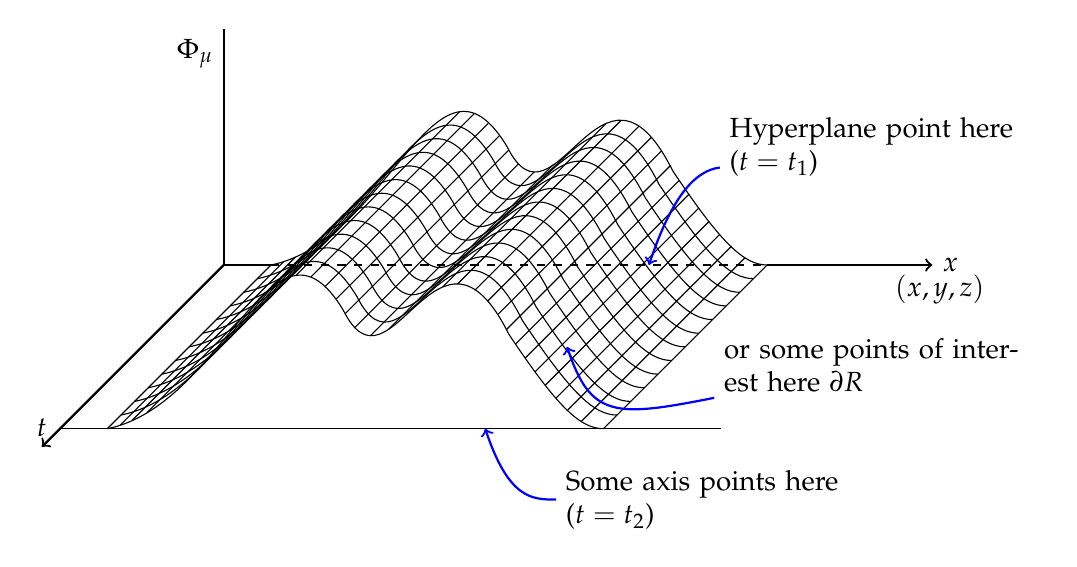
\begin{tikzpicture}[scale=3,block/.style={text width=11.2em}]
    % defining the coordinate axis
    \draw[thick] (0,0,0)--(0.2,0,0);
    \draw[dashed,thick] (0.2,0,0)--(2.3,0,0);
    \draw[->, thick] (2.3,0,0)--(3,0,0) node[right]{$x$};% x axis
    \draw[thick] (0,0,0)--(0,1,0) node[anchor=north east]{$\Phi_{\mu}$}; % field axis
    \draw[->,thick] (0,0,0)--(0,0,2) node[above]{$t$}; % t axis
    % draw the graphs
    \draw (0,0,1.8)--(2.8,0,1.8);
    \draw (0.2,0,1.8)--(0.2,0,0);
    \draw (2.3,0,1.8)--(2.3,0,0);
    \draw (0.2,0,0) .. controls (0.7,0.1,0) and (0.9,1,0) .. (1.2,0.5,0)
                    .. controls (1.4,0.1,0) and (1.6,1,0) .. (1.9,0.4,0)
                    .. controls (2.1,0.1,0) and (2.2,0.0,0) .. (2.3,0.0,0);
    \draw (0.2,0,0.15) .. controls (0.7,0.1,0.15) and (0.9,1,0.15) .. (1.2,0.5,0.15)
                    .. controls (1.4,0.1,0.15) and (1.6,1,0.15) .. (1.9,0.4,0.15)
                    .. controls (2.1,0.1,0.15) and (2.2,0.0,0.15) .. (2.3,0.0,0.15);
    \draw (0.2,0,0.3) .. controls (0.7,0.1,0.3) and (0.9,1,0.3) .. (1.2,0.5,0.3)
                    .. controls (1.4,0.1,0.3) and (1.6,1,0.3) .. (1.9,0.4,0.3)
                    .. controls (2.1,0.1,0.3) and (2.2,0.0,0.3) .. (2.3,0.0,0.3);
    \draw (0.2,0,0.45) .. controls (0.7,0.1,0.45) and (0.9,1,0.45) .. (1.2,0.5,0.45)
                    .. controls (1.4,0.1,0.45) and (1.6,1,0.45) .. (1.9,0.4,0.45)
                    .. controls (2.1,0.1,0.45) and (2.2,0.0,0.45) .. (2.3,0.0,0.45);
    \draw (0.2,0,0.6) .. controls (0.7,0.1,0.6) and (0.9,1,0.6) .. (1.2,0.5,0.6)
                    .. controls (1.4,0.1,0.6) and (1.6,1,0.6) .. (1.9,0.4,0.6)
                    .. controls (2.1,0.1,0.6) and (2.2,0.0,0.6) .. (2.3,0.0,0.6);
    \draw (0.2,0,0.75) .. controls (0.7,0.1,0.75) and (0.9,1,0.75) .. (1.2,0.5,0.75)
                    .. controls (1.4,0.1,0.75) and (1.6,1,0.75) .. (1.9,0.4,0.75)
                    .. controls (2.1,0.1,0.75) and (2.2,0.0,0.75) .. (2.3,0.0,0.75);
    \draw (0.2,0,0.9) .. controls (0.7,0.1,0.9) and (0.9,1,0.9) .. (1.2,0.5,0.9)
                    .. controls (1.4,0.1,0.9) and (1.6,1,0.9) .. (1.9,0.4,0.9)
                    .. controls (2.1,0.1,0.9) and (2.2,0.0,0.9) .. (2.3,0.0,0.9);
    \draw (0.2,0,1.05) .. controls (0.7,0.1,1.05) and (0.9,1,1.05) .. (1.2,0.5,1.05)
                    .. controls (1.4,0.1,1.05) and (1.6,1,1.05) .. (1.9,0.4,1.05)
                    .. controls (2.1,0.1,1.05) and (2.2,0.0,1.05) .. (2.3,0.0,1.05);
    \draw (0.2,0,1.20) .. controls (0.7,0.1,1.20) and (0.9,1,1.20) .. (1.2,0.5,1.20)
                    .. controls (1.4,0.1,1.20) and (1.6,1,1.20) .. (1.9,0.4,1.20)
                    .. controls (2.1,0.1,1.20) and (2.2,0.0,1.20) .. (2.3,0.0,1.20);
    \draw (0.2,0,1.35) .. controls (0.7,0.1,1.35) and (0.9,1,1.35) .. (1.2,0.5,1.35)
                    .. controls (1.4,0.1,1.35) and (1.6,1,1.35) .. (1.9,0.4,1.35)
                    .. controls (2.1,0.1,1.35) and (2.2,0.0,1.35) .. (2.3,0.0,1.35);
    \draw (0.2,0,1.5) .. controls (0.7,0.1,1.5) and (0.9,1,1.5) .. (1.2,0.5,1.5)
                    .. controls (1.4,0.1,1.5) and (1.6,1,1.5) .. (1.9,0.4,1.5)
                    .. controls (2.1,0.1,1.5) and (2.2,0.0,1.5) .. (2.3,0.0,1.5);
    \draw (0.2,0,1.65) .. controls (0.7,0.1,1.65) and (0.9,1,1.65) .. (1.2,0.5,1.65)
                    .. controls (1.4,0.1,1.65) and (1.6,1,1.65) .. (1.9,0.4,1.65)
                    .. controls (2.1,0.1,1.65) and (2.2,0.0,1.65) .. (2.3,0.0,1.65);
    \draw (0.2,0,1.8) .. controls (0.7,0.1,1.8) and (0.9,1,1.8) .. (1.2,0.5,1.8)
                    .. controls (1.4,0.1,1.8) and (1.6,1,1.8) .. (1.9,0.4,1.8)
                    .. controls (2.1,0.1,1.8) and (2.2,0.0,1.8) .. (2.3,0.0,1.8);

    \draw (0.25,0.01,1.785)--(0.25,0.01,-0.01);
    \draw (0.30,0.03,1.785)--(0.30,0.03,-0.01);
    \draw (0.35,0.05,1.755)--(0.35,0.05,0.7);
    \draw (0.43,0.13,0.56)--(0.43,0.13,0.17);
    \draw (0.48,0.13,0.45)--(0.48,0.13,-1.35);
    \draw (0.55,0.13,0.47)--(0.55,0.13,-1.33);
    \draw (0.65,0.13,0.57)--(0.65,0.13,-1.22);
    \draw (0.75,0.13,0.71)--(0.75,0.13,-1.08);
    \draw (0.85,0.13,0.87)--(0.85,0.13,-0.930);
    \draw (0.95,0.13,1.03)--(0.95,0.13,-0.775);
    \draw (1.05,0.13,1.115)--(1.05,0.13,-0.685);
    \draw (1.1,0.13,1.05)--(1.1,0.13,-0.765);
    \draw (1.15,0.13,0.58)--(1.15,0.13,-1.22);
    \draw (1.2,0.13,0.546)--(1.2,0.13,-1.25);
    \draw (1.3,0.13,0.616)--(1.3,0.13,-1.187);
    \draw (1.4,0.13,0.735)--(1.4,0.13,-1.065);
    \draw (1.5,0.13,0.88)--(1.5,0.13,-0.92);
    \draw (1.6,0.13,1.05)--(1.6,0.13,-0.76);
    \draw (1.7,0.13,1.21)--(1.7,0.13,-0.59);
    \draw (1.8,0.13,1.36)--(1.8,0.13,-0.44);
    \draw (1.9,0.13,1.51)--(1.9,0.13,-0.29);
    \draw (2.0,0.13,1.66)--(2.0,0.13,-0.14);
    \draw (2.1,0.13,1.8)--(2.1,0.13,0);
    \draw (2.15,0.08,1.8)--(2.15,0.08,0);
    \draw (2.196,0.02,1.77)--(2.196,0.02,-0.03);
% nodes: description of the regions and hypersurface
    \node[below right] at (2.8,0,0) {$\left(x,y,z\right)$};
    \path[block] (2.1,0.5,0) node[right] (x){Hyperplane point here ($t=t_{1}$)};
    \path[block] (2.1,-0.3,1.8) node[right] (y){Some axis points here ($t=t_{2}$)};
    \path[block] (2.5,0,1.1) node[right] (z){or some points of interest here $\partial R$};
    \draw[->,thick,blue] (x) .. controls (2.0,0.4,0) and (1.9,0.3,0) .. (1.8,0,0);
    \draw[->,thick,blue] (y) .. controls (2.0,-0.3,1.8) and (1.9,-0.3,1.8) .. (1.8,-0,1.8);
    \draw[->,thick,blue] (z) .. controls (2.0,-0.3,0.9) and (1.9,-0.3,0.9) .. (1.8,-0,0.9);
    
    \end{tikzpicture}
    \caption{Caption explaining significance of the image}
    \label{fig:my_label}
\end{figure}

\section{Mathematical Statements and Programs}

\begin{equation}
\frac{d\gamma}{dt} > 0,
\frac{d^2\alpha}{dt^2} > 0,
\forall t > 0.
\end{equation}

\end{sloppypar}
%\include{Chapters/Chapter4} 
%\include{Chapters/Chapter5} 

\end{spacing}

%----------------------------------------------------------------------------------------
%	THESIS CONTENT - APPENDICES
%----------------------------------------------------------------------------------------

\appendix % Cue to tell LaTeX that the following "chapters" are Appendices

% Include the appendices of the thesis as separate files from the Appendices folder
% Uncomment the lines as you write the Appendices

% Appendix A

\chapter{Frequently Asked Questions} % Main appendix title

\label{AppendixA} % For referencing this appendix elsewhere, use \ref{AppendixA}

\section{How do I change the colors of links?}

The color of links can be changed to your liking using:

{\small\verb!\hypersetup{urlcolor=red}!}, or

{\small\verb!\hypersetup{citecolor=green}!}, or

{\small\verb!\hypersetup{allcolor=blue}!}.

\noindent If you want to completely hide the links, you can use:

{\small\verb!\hypersetup{allcolors=.}!}, or even better: 

{\small\verb!\hypersetup{hidelinks}!}.

\noindent If you want to have obvious links in the PDF but not the printed text, use:

{\small\verb!\hypersetup{colorlinks=false}!}.

%\include{Appendices/AppendixB}
%\include{Appendices/AppendixC}

%----------------------------------------------------------------------------------------
%	BIBLIOGRAPHY
%----------------------------------------------------------------------------------------

\printbibliography[heading=bibintoc]

%----------------------------------------------------------------------------------------
\end{sloppypar}
\end{document}  
